\chapter{Development Plan}
\label{chap:Chapter5}
%-------------------------------------------------------------------------------%
\section{Research Approach}
To achieve the desired objectives and system requirements, the development approach will be composed of three phases: Dissertation Development, System Development, and Implementation.

To gain an improved understanding of the present status of the subject, a study of the literature on fixed-pitch propellers, UAV propulsion systems, and new developments in VPP technology will be conducted during the first part of dissertation development.
Analyzing earlier VPP deployments in UAVs will yield insightful information on successful examples, difficulties encountered, and lessons discovered, advancing our knowledge of real-world applications.
The research plan includes a methodical approach to solving the issue at hand, as well as a thorough development strategy, system architecture, goals and objectives description, requirements definition, and problem analysis.The next stage, called "Result Analysis and Conclusions," will entail compiling and assessing the results of previous implementations and making judgments on the effectiveness of VPP systems in getting over fixed-pitch constraints.

As we go on to the System Development phase, detailed procedures are provided for acquiring parts, creating schematics and printed circuit boards (PCBs), producing PCBs, and creating firmware for crucial parts like the Real-Time Clock (RTC) and On-Board Computer (OBC).
To guarantee optimal operation, the strategy incorporates a crucial stage for firmware validation and modulation.

Building the Main and Secondary Devices, doing bench and ground tests, and methodically assessing the VPP system in comparison to predetermined goals and criteria are all part of the ensuing Implementation phase.
Dissertation Development

1. State of the Art
In this phase, a thorough review of existing literature on UAV propulsion systems, fixed-pitch propellers, and recent advancements in Variable Pitch Proprotor (VPP) systems will be conducted. 
This will provide a foundation for understanding the current landscape and challenges.

2. Describe Implementations
The research will analyze and document existing implementations of VPP systems in UAVs. 
By highlighting successful cases, challenges faced, and lessons learned, the study aims to gain insights into the practical applications of VPP technology.

3. Result Analysis and Conclusions
Summarizing and analyzing the results of the described implementations will form a critical part of the research. 
Conclusions will be drawn regarding the effectiveness of VPP systems in overcoming the limitations associated with fixed-pitch propellers.

4. Research Plan
This section will define the methodology for addressing the research problem. 
Specific steps and activities will be outlined to achieve the research objectives. 
Key components include problem analysis, requirements definition, goals and objectives definition, system architecture definition, system flow chart, and a detailed development plan.

System Development

1. Component Procurement
Identifying and sourcing the necessary components for the VPP system will be a crucial step in the development process.

2. Schematic and PCB Design
Detailed schematics and PCB layouts for both the Main Device Unit (MDU) and Secondary Device Units (SDUs) will be created.

3. PCB Manufacture and Component Acquisition
This step involves the actual manufacturing of PCBs based on the designed schematics and acquiring all the necessary components for the assembly process.

4. Firmware Development
Firmware for essential components like the On-Board Computer (OBC), Real-Time Clock (RTC), and wireless communication modules will be developed.

5. Firmware Validation and Modulation
Validation of the developed firmware through simulations and testing will be carried out.
Any necessary adjustments or modulations to enhance performance will be implemented.

Implementation

1. Build Main and Secondary Device
Assembling the MDU and SDUs, integrating the developed PCBs and components to create functional devices.

2. Bench Tests
Conducting initial bench tests to evaluate the functionality of individual components and their interactions.

3. Ground Tests
Performing comprehensive ground tests to assess the overall functionality of the VPP system in a controlled environment.

4. Evaluation
Systematically evaluating the VPP system against predefined requirements and objectives.
Documenting results and making any necessary refinements to enhance performance.



%-------------------------------------------------------------------------------%

\section{Evaluation}
COM
- Stable
- Low latency

Propeller Control
- Stable Control
- Fail-safe mechanism

Control
- quick response to change in flight phase and Maneuver
- quick response in error scenarios

FIRMWARE
- flow modulation and verification
%-------------------------------------------------------------------------------%

\section{Timeline}



\begin{figure}[H]
    \centering
    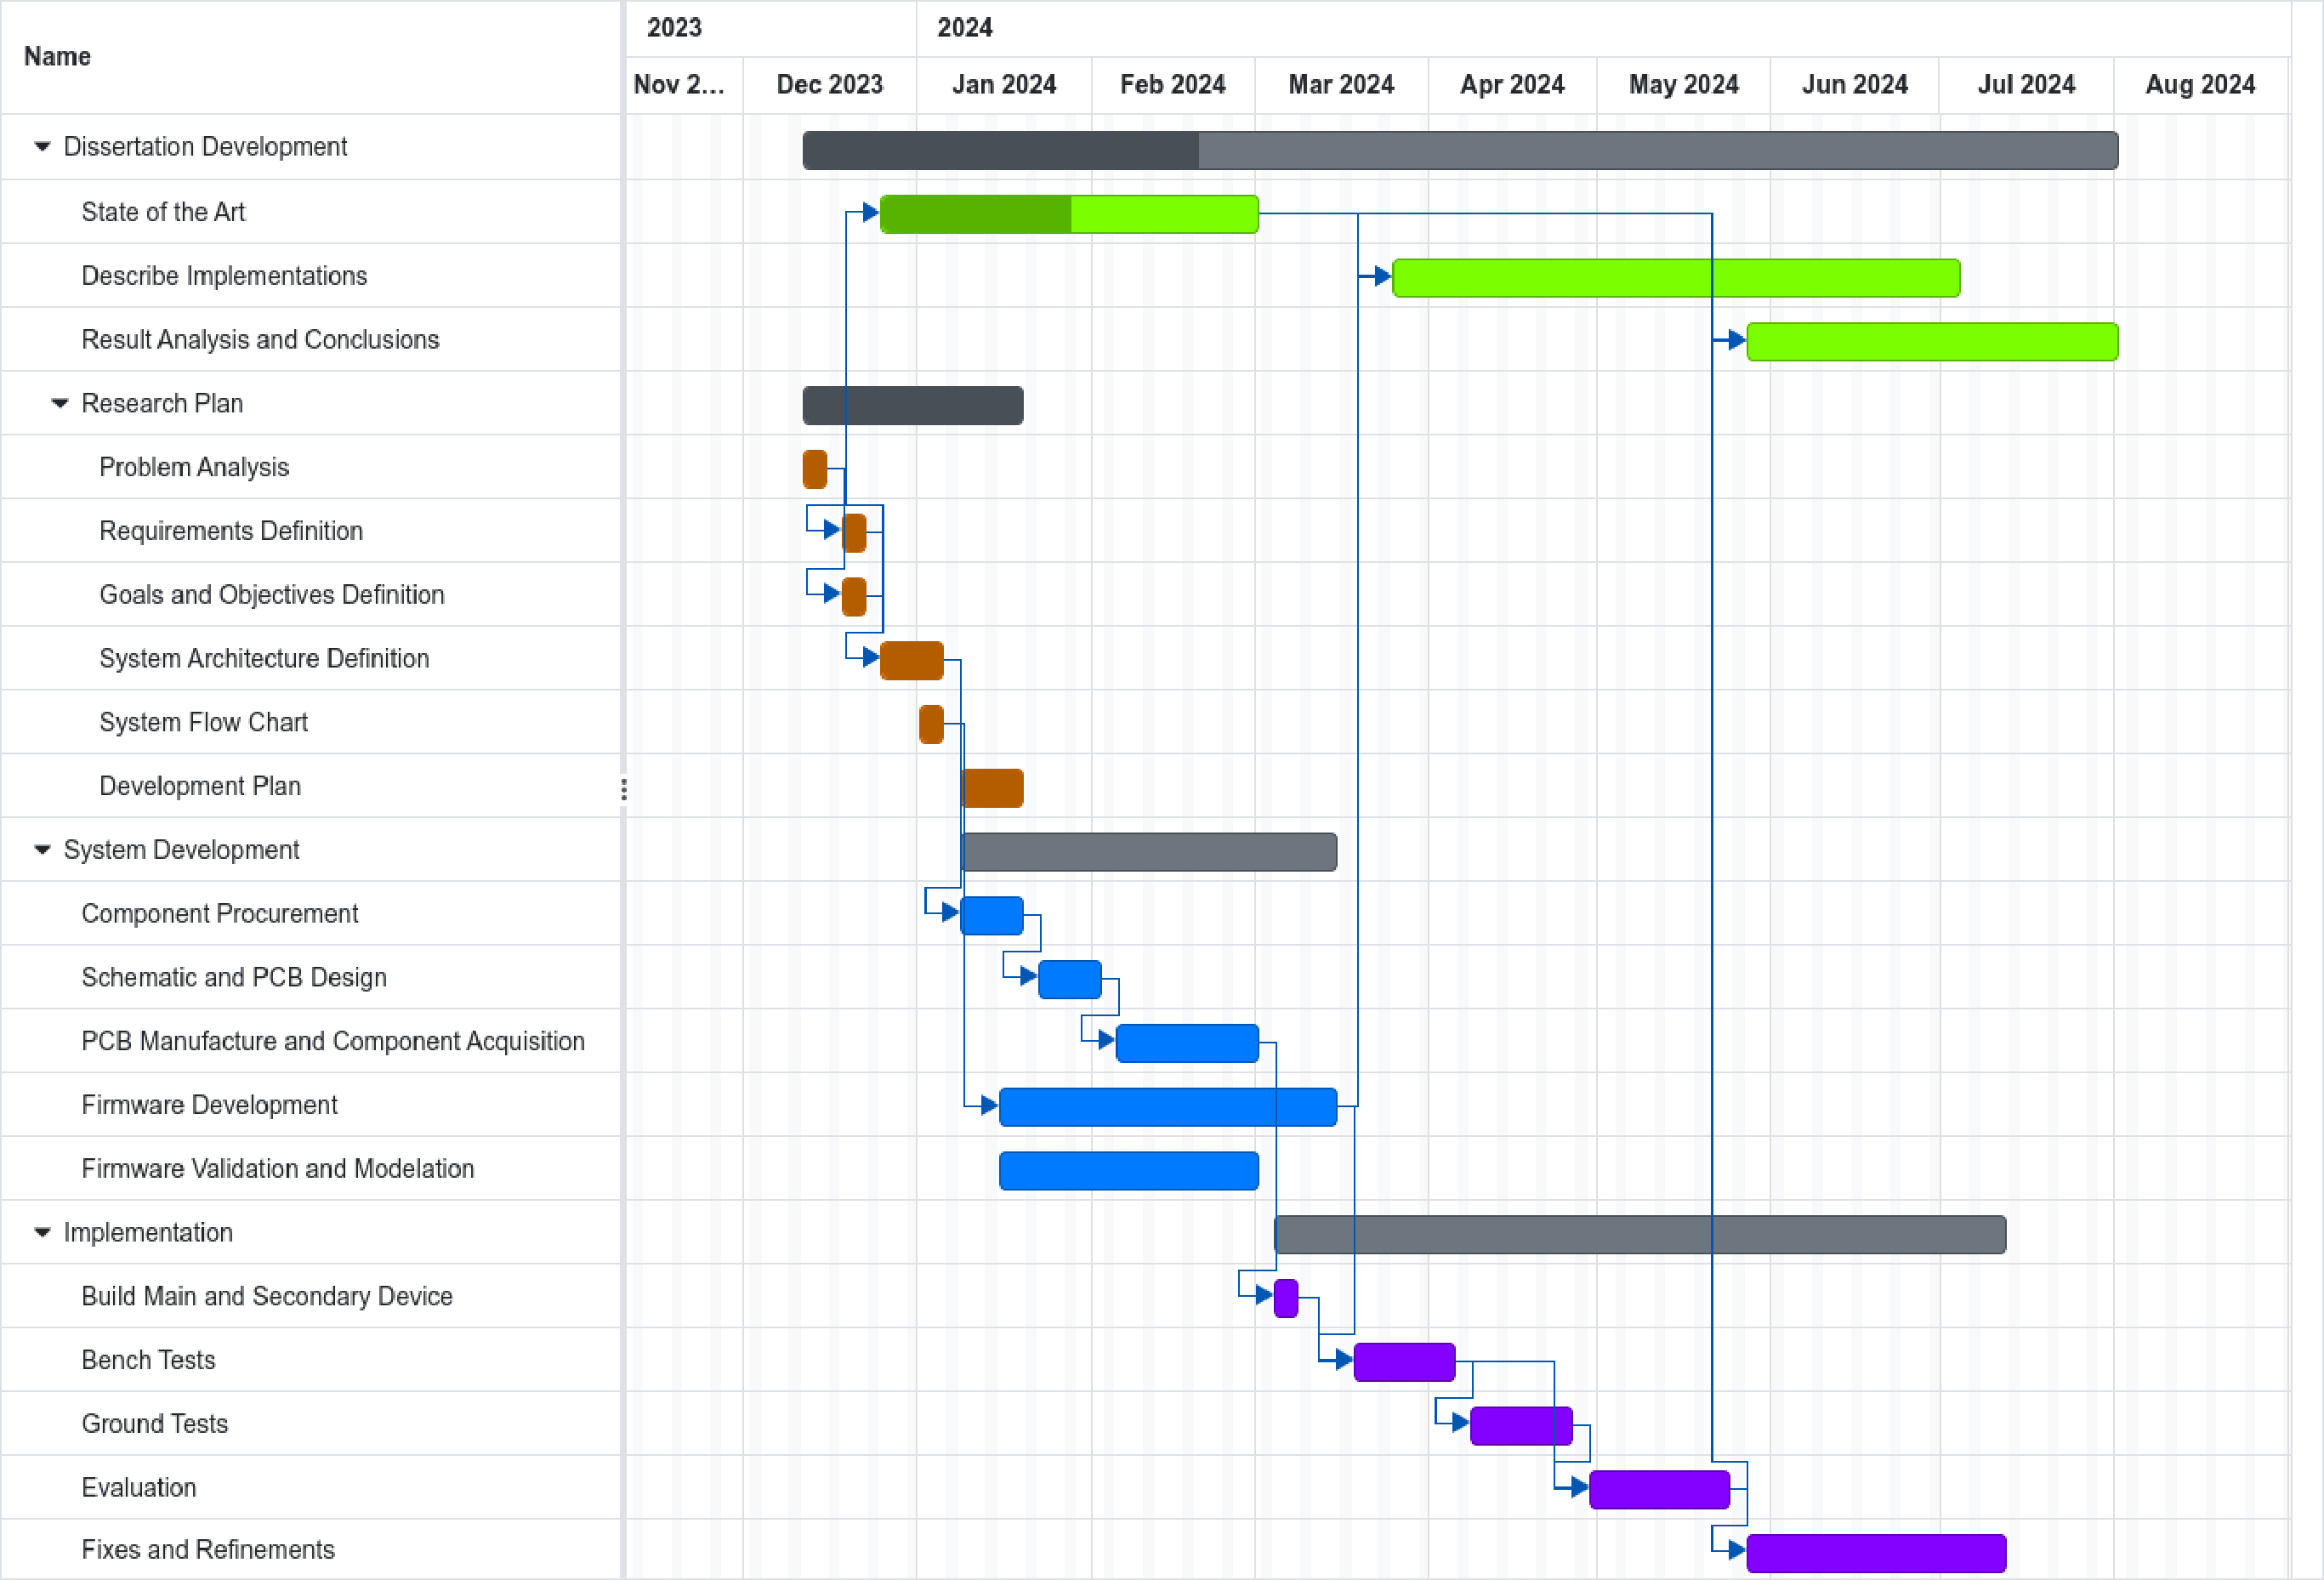
\includegraphics[width=\textwidth,keepaspectratio]{ch5/assets/gantt.pdf}
    \caption{Project timeline Gantt chart}
    \label{gantt}
\end{figure}